\documentclass[tikz,border=2mm]{standalone}
\usetikzlibrary{calc,quotes,intersections, angles}

\begin{document}
    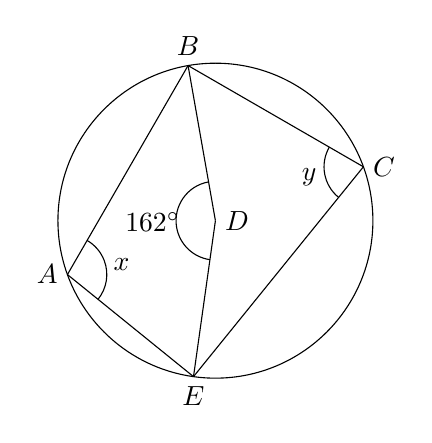
\begin{tikzpicture}[scale=2]
    %mark points on circle
        \coordinate[label = right:$D$] (D) at (0,0);
        \coordinate[label=left:$A$] (A) at (200:1);
        \coordinate[label=above:$B$] (B) at (100:1);
        \coordinate[label=right:$C$] (C) at (20:1);
        \coordinate[label=below:$E$] (E) at (262:1);

    %draw chords and circle
        \draw[name path=circ] (0,0) circle (1);
        \draw (B) -- (D);
        \draw (D) -- (E);
        \draw (B) -- (C);
        \draw (E) -- (C);
        \draw (A) -- (B);
        \draw (A) -- (E);
      
        \pic [draw, "$162^\circ$", angle eccentricity=1.6, angle radius = 0.5cm] {angle = B--D--E};
        \pic [draw, "$x$", angle eccentricity=1.4, angle radius = 0.5cm] {angle = E--A--B};
        \pic [draw, "$y$", angle eccentricity=1.4, angle radius = 0.5cm] {angle = B--C--E};
        % \pic [draw, "$x$", angle eccentricity=1.3, angle radius = 0.5cm] {angle = C--D--B};
        
    \end{tikzpicture}
\end{document}